% Für Seitenformatierung

\documentclass[DIV=15]{scrartcl}

% Zeilenumbrüche

\parindent 0pt
\parskip 6pt

% Für deutsche Buchstaben und Synthax

\usepackage[ngerman]{babel}

% Für Auflistung mit speziellen Aufzählungszeichen

\usepackage{paralist}

% zB für \del, \dif und andere Mathebefehle

\usepackage{amsmath}
\usepackage{commath}
\usepackage{amssymb}

% Für \SIunit[]{} und \num in deutschem Stil

\usepackage[output-decimal-marker={,}]{siunitx}

% Schriftart und encoding

\usepackage[utf8]{inputenc}
\usepackage[charter, greekuppercase=italicized]{mathdesign}
\usepackage{beramono}

% Für \sfrac{}{}, also inline-frac

\usepackage{xfrac}

% Für Einbinden von pdf-Grafiken

\usepackage{graphicx}

% Umfließen von Bildern

\usepackage{floatflt}

% Für Links nach außen und innerhalb des Dokumentes

\usepackage{hyperref}

% Für weitere Farben

\usepackage{color}

% Für Streichen von z.B. $\rightarrow$

\usepackage{centernot}

% Für Befehl \cancel{}

\usepackage{cancel}

% Für Layout von Links

\hypersetup{
	citecolor=black,
	colorlinks=true,
	linkcolor=black,
	urlcolor=blue,
}

% Verschiedene Mathematik-Hilfen

\newcommand \e[1]{\cdot10^{#1}}
\newcommand\p{\partial}

\newcommand\half{\frac 12}
\newcommand\shalf{\sfrac12}

\newcommand\skp[2]{\left\langle#1,#2\right\rangle}
\newcommand\mw[1]{\left\langle#1\right\rangle}
\newcommand \eexp[1]{\mathrm{e}^\del{#1}}
\newcommand \dexp[1]{\exp\del{#1}}

% Nabla und Kombinationen von Nabla

\renewcommand\div[1]{\skp{\nabla}{#1}}
\newcommand\rot{\nabla\times}
\newcommand\grad[1]{\nabla#1}
\newcommand\laplace{\triangle}
\newcommand\dalambert{\mathop{{}\Box}\nolimits}

%Für komplexe Zahlen

\newcommand \ii{\mathrm i}
\renewcommand{\Im}{\mathop{{}\mathrm{Im}}\nolimits}
\renewcommand{\Re}{\mathop{{}\mathrm{Re}}\nolimits}

%Für Bra-Ket-Notation

\newcommand\bra[1]{\left\langle#1\right|}
\newcommand\ket[1]{\left|#1\right\rangle}
\newcommand\braket[2]{\left\langle#1\left.\vphantom{#1 #2}\right|#2\right\rangle}
\newcommand\braopket[3]{\left\langle#1\left.\vphantom{#1 #2 #3}\right|#2\left.\vphantom{#1 #2 #3}\right|#3\right\rangle}


\setcounter{section}{0}
\renewcommand\thesection{H\,7.\arabic{section}}
\renewcommand\thesubsection{\thesection.\alph{subsection}}

\title{physik521: Übungsblatt 07}
\author{%
    Lino Lemmer \\ \small{\texttt{s6lilemm@uni-bonn.de}}
    \and
    Martin Ueding \\ \small{\texttt{mu@martin-ueding.de}}
    \and
    Paul Manz \\ \small{\texttt{p.m@uni-bonn.de}}
}

\begin{document}
\maketitle
\section{Zweiatomiges Molekül}

\section{Kühlung durch adiabatische Entmagnetisierung}

\subsection{Entropie}

Hier ist nach der kanonischen Zustandssumme gefragt, daher betrachten wir dieses System auch im kanonischen Formalismus. Wir bestimmen $Z_\text C$:
\begin{align*}
    Z_\text C
    &= \prod_{i=1}^N \sum_{s_i = -1, 0, 1} \exp\del{\frac{\mu B s_i}{k T}} \\
    &= \del{\sum_{s_i = -1, 0, 1} \exp\del{\frac{\mu B s_i}{k T}}}^N \\
    &= \del{1 + 2 \cosh\del{\frac{\mu B s_i}{k T}}}^N.
\end{align*}

Daraus können wir die freie Energie $F(T) = - k T \ln(Z_\text C)$ bestimmen:
\[
    F(T) = - N k T \ln\del{1 + 2 \cosh\del{\frac{\mu B s_i}{k T}}}.
\]

Aus der freien Energie bestimmen wir die Entropie:
\begin{align*}
    S(T)
    &= - \dpd FT \\
    &= N k \del{
        \ln\del{1 + 2 \cosh\del{\frac{\mu B s_i}{k T}}}
        - \frac{\mu B}{kT} \frac{2 \sinh\del{\frac{\mu B s_i}{k T}}}{1 + 2\cosh\del{\frac{\mu B s_i}{k T}}}
    }.
\end{align*}

Dies stimmt mit dem Kontrollergebnis überein.

\subsection{Abkühlung}

Die Temperatur wird auf $T_1$ fixiert. Wenn es adiabatisch geändert wird, ist
$\deltaup Q = 0$. Außerdem geht es so schnell, dass die Teilsysteme sich nicht
verändern können. $W_\text C$ bleibt also fest. Daher muss auch $Z_\text C$
sowie $F$ und $S$ konstant bleiben.

\subsection{Neue Temperatur}

Wir haben es nicht geschafft, analytisch zu zeigen, dass $S(T)$ injektiv ist.
Dies bedeutet, dass zwei verschiedene Entropien durch zwei verschiedene $B/T$
kommen muss. Als Anschauung haben wir zwei Plots erstellt, in denen Qualitativ
$S(B/T)$ und die Ableitung $S'(B/T)$ geplottet worden sind:

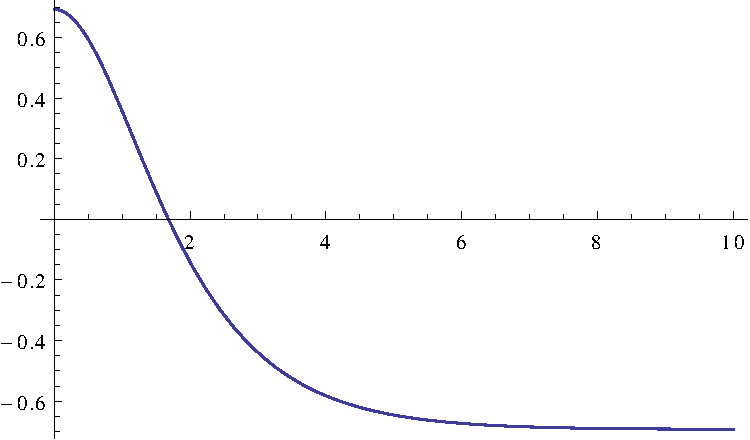
\includegraphics[width=.45\textwidth]{2b-S.pdf}
\hfill
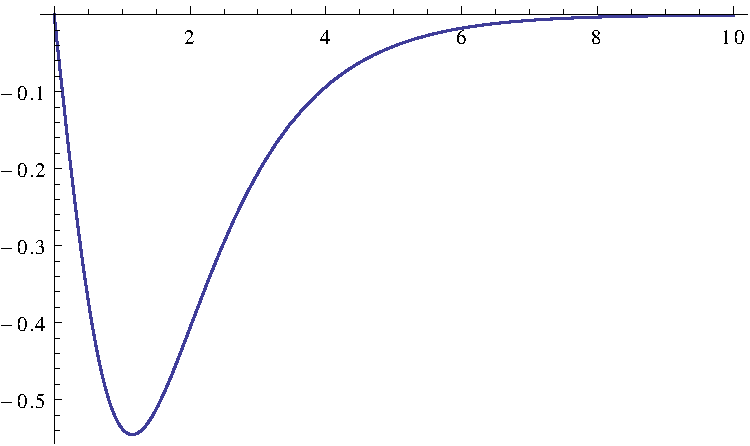
\includegraphics[width=.45\textwidth]{2b-dS.pdf}

Es ist zu sehen, dass die Funktion streng monoton falled ist, die Ableitung ist
immer negativ. Daher ist die Funktion sogar bijektiv, also auch injektiv.

Es muss
\[
    \frac{B_1}{T_1} = \frac{B_2}{T_2}
\]
gelten, da $S$ konstant ist, $S$ injektiv ist und daher $\mu B/kT$ konstant
sein muss.

Man muss $B_2 < B_1$ wählen, damit es passt.

\section{Polymer-Modell (Gummi)}

\end{document}
